% -----------------------------------------------
% Template for JIM
%     jim.sty -> style file
% By Eloi Batlle (eloi@iua.upf.es), changes for 
% ICMC by Bram de Jong (bdejong@iua.upf.es)
% changes for JIM 2007 by Dominique Fober (fober@grame.fr)
% changes for JIM 2009 by Olivier Tache (olivier.tache@imag.fr)
% -----------------------------------------------

\documentclass{article}
\usepackage{jim}
\usepackage[utf8]{inputenc}
\usepackage[francais]{babel}
\usepackage[T1]{fontenc}
\usepackage{graphicx}
\usepackage{amssymb,amsmath} 
\usepackage{balance}

\usepackage{color}
\usepackage{hyperref}
\usepackage[nocenter]{qtree}
\usepackage{tree-dvips}
\usepackage{listings}

\definecolor{lightgrey}{rgb}{0.95,0.95,0.95}
\definecolor{mycolor}{rgb}{0.0,0.0,0.8}
\hypersetup{
	colorlinks=true,
	citecolor = mycolor,
	linkcolor = mycolor,
	urlcolor  = mycolor
}

\definecolor{lightgrey}{rgb}{0.97,0.97,0.97}

\newcommand{\IS}		{INScore}
\newcommand{\exemple}	{\vspace*{2mm}\hspace*{-4mm}\textbf{Exemple :}}

\newcommand{\code}	[2][0.9]	{\vspace{0mm}\begin{center}\colorbox{lightgrey}{
							\begin{minipage}[t]{#1\columnwidth} 
							{\small \texttt{#2}}
							\end{minipage}}\end{center}}

\newcommand{\llist}	[1]		{\ensuremath{[#1_1,...,#1_k]}}

\newcommand{\type}		{\ensuremath{{\scriptsize \texttt{type}}}}
\newcommand{\seq}		{\ensuremath{|}}
\newcommand{\paral}		{\ensuremath{\parallel}}
\newcommand{\forest}	{\ensuremath{\varnothing}}
\newcommand{\toType}	{\ensuremath{\mathcal{T}}}
%\newcommand{\toAddress}	{\ensuremath{\text{@}}}
\newcommand{\toAddress}	{\ensuremath{\varGamma}}
\newcommand{\toOSCAddress}	{\ensuremath{{\scriptsize \texttt{OSC}}}}
\newcommand{\taddress}	{\ensuremath{\text{@}}}
\newcommand{\toData}	{\ensuremath{\text{D}}}
\newcommand{\tdata}	    {\ensuremath{\text{D}}}
\newcommand{\binop}		{\ensuremath{\texttt{op}}}
\newcommand{\etc}		{\ensuremath{\text{…}}}
\newcommand{\emptyf}	{\ensuremath{[\ ]}}

\newcommand{\nexpand}	{\ensuremath{\varepsilon}}
\newcommand{\ula}		{\hspace*{8mm}}
\newcommand{\ulb}		{\hspace*{31.5mm}}
\newcommand{\ulc}		{\hspace*{5.7mm}}
\newcommand{\uld}		{\hspace*{9mm}}


% Title.
% ------
\title{Un langage basé sur des arbres pour la description de partitions musicales}

% Single \textsc{address}
% To use with only one author or several with the same address
% ---------------
\oneauthor
  {D. Fober \quad Y. Orlarey \quad S. Letz \quad R. Michon} {Grame-CNCM \\
  Lyon - France \\
     {\tt {\small \{fober, orlarey, letz, michon\}@grame.fr}}}


\begin{document}
%
\maketitle
%
%-------------------------------------------------
\begin{abstract}
Le travail présenté s'inscrit dans le projet \IS, un environnement pour la conception de partition interactives augmentées, tourné vers des usages non conventionnels de la notation et de la représentation de la musique, sans exclure pour autant les approches classiques. Cet environnement est entièrement pilotable par des messages Open Sound Control [OSC]. Un langage de script, basé sur une version textuelle étendue de ces messages permet de concevoir des partitions sous forme modulaire et incrémentale. Cet article présente une révision majeure de ce langage de script, fondée sur la description et la manipulation d'arbres.
\end{abstract}

%-------------------------------------------------
\section{Introduction}\label{sec:introduction}

Il existe un grand nombre de langages de description de partitions musicales (Lilypond \cite{lilypond03}, Guido \cite{hoos98}, MuseData \cite{Hewlett97}, MEI \cite{Roland_2002}, MusicXML \cite{good01} etc.), tous axés sur une notation symbolique occidentale.
 
Certains de ces langages ont été étendus, afin de leur ajouter de la \textit{programmabilité}, comme par exemple des opérations de composition de partitions musicales dans Guido \cite{fober12b}, ou le langage Scheme dans Lilypond.
Il existe aussi des langages de programmation dédiés à la notation musicale commune, comme CMN \cite{Schottstaedt97} ou ENP 
qui sont en fait des dialectes de Lisp.

L'approche proposée par \IS\ \cite{Fober:12a} est assez différente : la notation musicale symbolique est supportée (via le langage et le moteur de rendu Guido \cite{Dau:09b,hoos98}), mais elle constitue un des moyens de représentation musicale parmi d'autres, sans être privilégiée. 
Des partitions purement graphiques peuvent être conçues. Tous les éléments d'une partition (y compris les éléments purement graphiques) ont une dimension temporelle (date, durée et tempo) et peuvent être manipulés dans l'espace graphique et temporel. La notion de temps est à la fois événementielle et continue \cite{fober17c}, ce qui permet de concevoir des partitions interactives et dynamiques. La figure \ref{pavlos} présente un exemple d'une partition réalisée avec \IS . Elle inclut de la notation symbolique, des images, une vidéo et des curseurs (la vidéo en est un) dont les positions sont synchronisées par les gestes de l'interprète.

\begin{figure}
\begin{center}
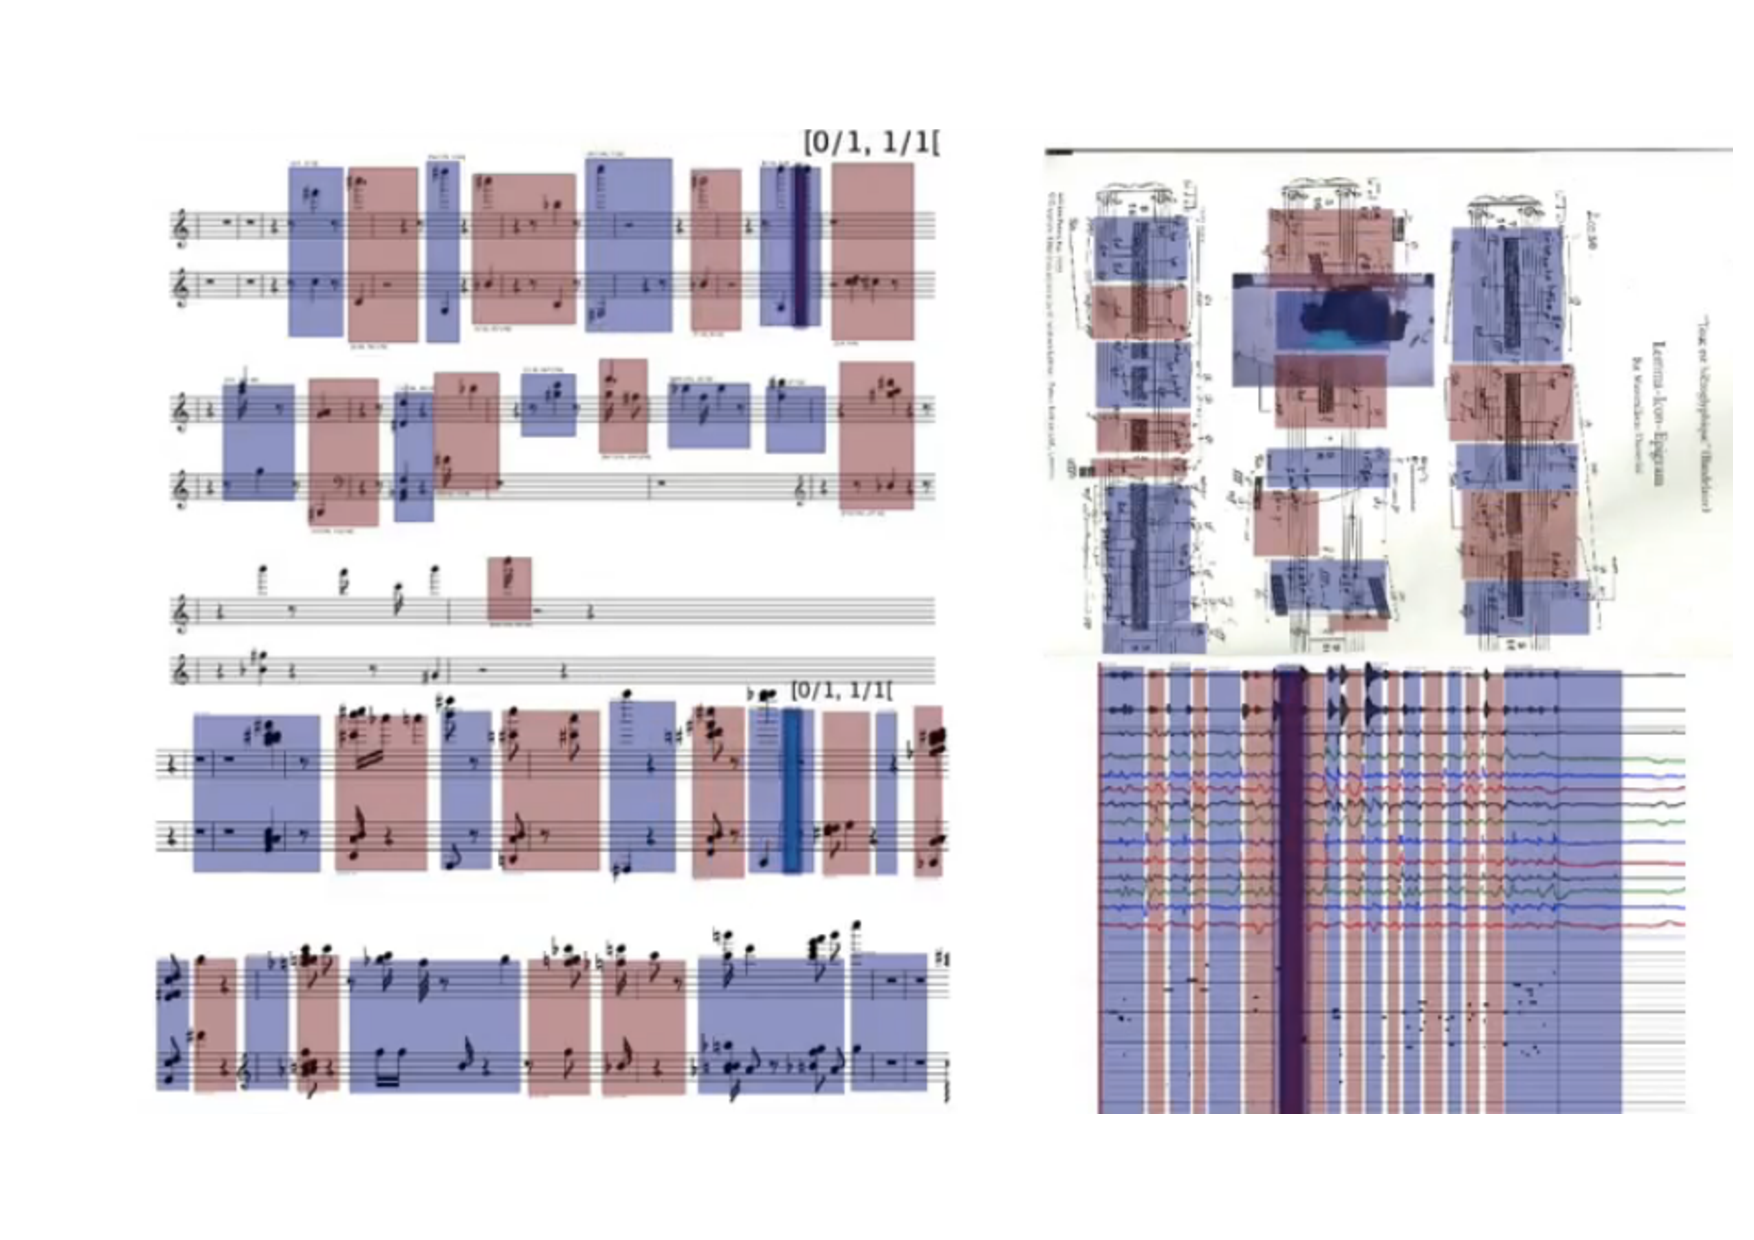
\includegraphics[width=0.98\columnwidth]{imgs/inscore-score}
\caption{Une partition réalisée avec \IS , utilisée dans le cadre d'un environnement basé sur des capteurs, dédié au traitement et à l'apprentissage de musiques complexes appelé \emph{GesTCom} (\emph{Gesture Cutting through Textual Complexity}) \cite{antoniadis:tel-01861171}.}
\label{pavlos}
\end{center}
\end{figure}

\IS\ a été initialement conçu pour être piloté par des messages OSC \cite{OSC}. OSC est conçu un protocole de communication. Une version textuelle des messages OSC constitue le format de stockage d'\IS, qui a été étendu en un langage de script, \cite{Fober:13b} permettant une plus grande flexibilité dans la conception des partitions musicales.
Ces extensions (variables, adresses étendues, section Javascript, etc.) souffrent néanmoins d'une rigidité inhérente à une conception ad hoc et incrémentale. Par exemple, l'analyseur syntaxique fait une distinction claire entre les adresses OSC et les données associées, ce qui empêche l'utilisation de variables dans les adresses OSC.
Une révision majeure de ce langage s'est donc avérée nécessaire. Elle est basé sur la manipulation d'une structure arborescente régulière qui est également homogène au modèle d'\IS.
La figure \ref{tree1} donne un exemple d'une telle hiérarchie du modèle, qui peut être décrite dans le langage de script courant (i.e. OSC) en listant toutes les branches à de l'arbre à partir de la racine. (Figure~\ref{script1})

\begin{figure}[htbp]
\begin{center}
\Tree [ .ITL [ .scene 
	[ .obj1 [ .x 0 ] [ .y 0 ] [ .date 0 ] ] 
	[ .obj2 [ .x 0.5 ] [ .y 0.5 ] [ .date 1 ] ] ] 
]
\caption{Exemple d'une partition \IS\ comprenant 2 objets $obj1$ et $obj2$, qui possèdent des attributs $x$, $y$, et $date$. Les feuilles de l'arbre sont les valeurs des attributs.}
\label{tree1}
\end{center}
\end{figure}

\begin{figure}[htbp]
\code{/ITL/scene/obj1 x 0;\\
/ITL/scene/obj1 y    0;\\
/ITL/scene/obj1 date 0;\\
/ITL/scene/obj2 x    0.5;\\
/ITL/scene/obj2 y    0.5;\\
/ITL/scene/obj2 date 1;
}
\caption{Script qui décrit la partition en figure \ref{tree1}.}
\label{script1}
\end{figure}

Aucune de ces approches ne couvre l'angle très particulier que nous avons adopté : celui d'un langage de description de partitions musicales basé sur la structure hiérachique à la fois de la partition et des messages OSC.

Après quelques définitions, nous présenterons les opérations élémentaires sur les arbres ainsi que la grammaire correspondante. Nous introduirons ensuite les opérations mathématiques sur les arbres, les concepts de \emph{variables} et de \emph{valeurs expansées}, et nous présenterons enfin la transformation de ce langage en messages OSC classiques avant de conclure.



%-------------------------------------------------
\section{Définitions}

Un arbre $t$ est constitué d'une valeur $v$ (d'un certain type de données) et de la liste (éventuellement vide) de ses sous-arbres.
\[
	t :  v \times \llist{t} 
\]

Un arbre avec une liste de sous-arbres vide $t:v\times \emptyf$ s'appelle une feuille. \\
Une valeur est soit une valeur littérale (i.e. texte, nombre) soit une valeur spéciale parmi les types suivants :
\begin{itemize}
\item forêt (\forest) : désigne un arbre comprenant uniquement des sous-arbres,
\item operator mathématique : indique une opération mathématique entre sous-arbres,
\item variable : désigne un arbre dont la valeur fait référence à un autre arbre, 
\item expand : indique un arbre à développer,
\item slash (/) : utilisé pour la conversion en OSC
\end{itemize}
L'utilisation et l'évaluation de ces valeurs sont détaillées dans les sections suivantes.


%-------------------------------------------------
\section{Operations sur les arbres}

Nous définissons deux opérations abstraites sur les arbres : la mise en séquence et en parallèle. Ces opérations n'ont pas de sémantique musicale, ni d'un point de vue temporel, ni d'un point de vue graphique. Elles sont définies comme des méthodes de construction algorithmique de messages OSC et opèrent sur l'organisation topologique des arbres. 

%-----------------------------
\subsection{Mise en séquence}
Mettre deux arbres $t$ et $t'$ en séquence consiste à ajouter $t'$ comme enfant de toutes les feuilles de $t$.
Nous noterons \seq\ l'opération de mise en séquence. \\
Soit 2 arbres $t : v \times \llist{t}$ et $t'$. Alors :
\[
	v \times \llist{t}\ \seq\ t'  \to  v  \times [t_1 \seq\ t',\etc, t_k \seq\ t']
\]
avec: 
\[
\left\{
\begin{array}{l}
	v \times \emptyf\ \seq\ t'  \to  v  \times [ t' ]\\
	v \times \emptyf\ \seq\ \forest \times \llist{t}  \to  v  \times \llist{t}\\
\end{array}
\right.
\]
La flèche droite ($\to$) indique le résultat de l'évaluation d'une expression.

%-----------------------------
\subsection{Mise en parallèle}
Mettre deux arbres $t$ et $t'$ en parallèle consiste à les mettre dans une même forêt.
Nous noterons \paral\ l'opération de mise en parallèle. 
Soit 2 arbres $t$ et $t'$ :
\[
	t \paral\ t'  \to  \forest \times [ t, t' ]
\]
Le résultat est un arbre dont la valeur \forest\ denote une forêt. \\
La parallelisation appliquée à une forêt préserve l'ordre des sous-arbres:
\[
\left\{
\begin{array}{l}
	\forest \times \llist{t}\  \paral\ t'  \to  \forest \times [t_1,\etc,t_k,t']\\
	t' \paral\ \forest \times \llist{t}\   \to  \forest \times [t',t_1,\etc,t_k]\\
\end{array}
\right.
\]


%-------------------------------------------------
\section{Grammaire}\label{agram}

Un arbre est syntactiquement définit en BNF comme suit :
\code{tree := value      \hspace*{8mm} $\to$ t := value \emptyf \\
\ula | tree tree         \hspace*{4mm} $\to$ t := tree \seq\ tree \\
\ula | / tree            \hspace*{9.7mm} $\to$ t := '/' \seq\ tree\\
\ula | tree , tree       \hspace*{0mm}  $\to$ t := tree \paral\ tree \\
\ula | ( tree )          \hspace*{6mm} $\to$ t := tree \\
\ula ;
}
La flèche droite ($\to$) indique l'arbre créé pour chaque con-struction syntactique. 
L'arbre dont la valeur est \emph{slash} (/) joue un rôle spécial dans la conversion en messages OSC. Ce rôle est décrit en section \ref{ssec:slash}.


%-------------------------------------------------
\section{Valeurs et évaluation}\label{sec:valeurs}

Cette section décrit comment sont évalués les arbres ayant les valeurs spéciales \emph{opérateur mathématique}, \emph{variable} et \emph{expand}.

%---------------------------
\subsection{Opérateurs mathématiques}

Les opérations mathématiques sur des arbres sont vues comme des opérations qui portent sur leurs valeurs tout en conservant les sous-arbres. Ces opérations comprennent les opérations arithmétiques et logiques, les fonctions trigonométriques et hyperboliques, les fonctions exponentielles et logarithmiques, la puissance, la racine carrée, etc.

Nous désignerons ces opérations par \binop. Puis pour 2 arbres $t : v \times \llist{t}$ et $t' : v' \times \llist{t'}$ :
\[
	\binop \times [ t, t']  \to  (\binop\ v\ v') \times [ t_1,\etc,t_k,t'_1,\etc,t'_k ]
\]


\exemple

Le script en figure~\ref{parsesample2} genère l'arbre illustré en figure \ref{treesample2} après évaluation des opérations mathématiques.
\begin{figure}[htbp]
\code{/A (b ((* (math.sin 1), 2))),\\
\ulc (c (math.pow 2.2, 0.4)),\\
\ulc (d (math.max 1, 2, 3));}
\begin{center}
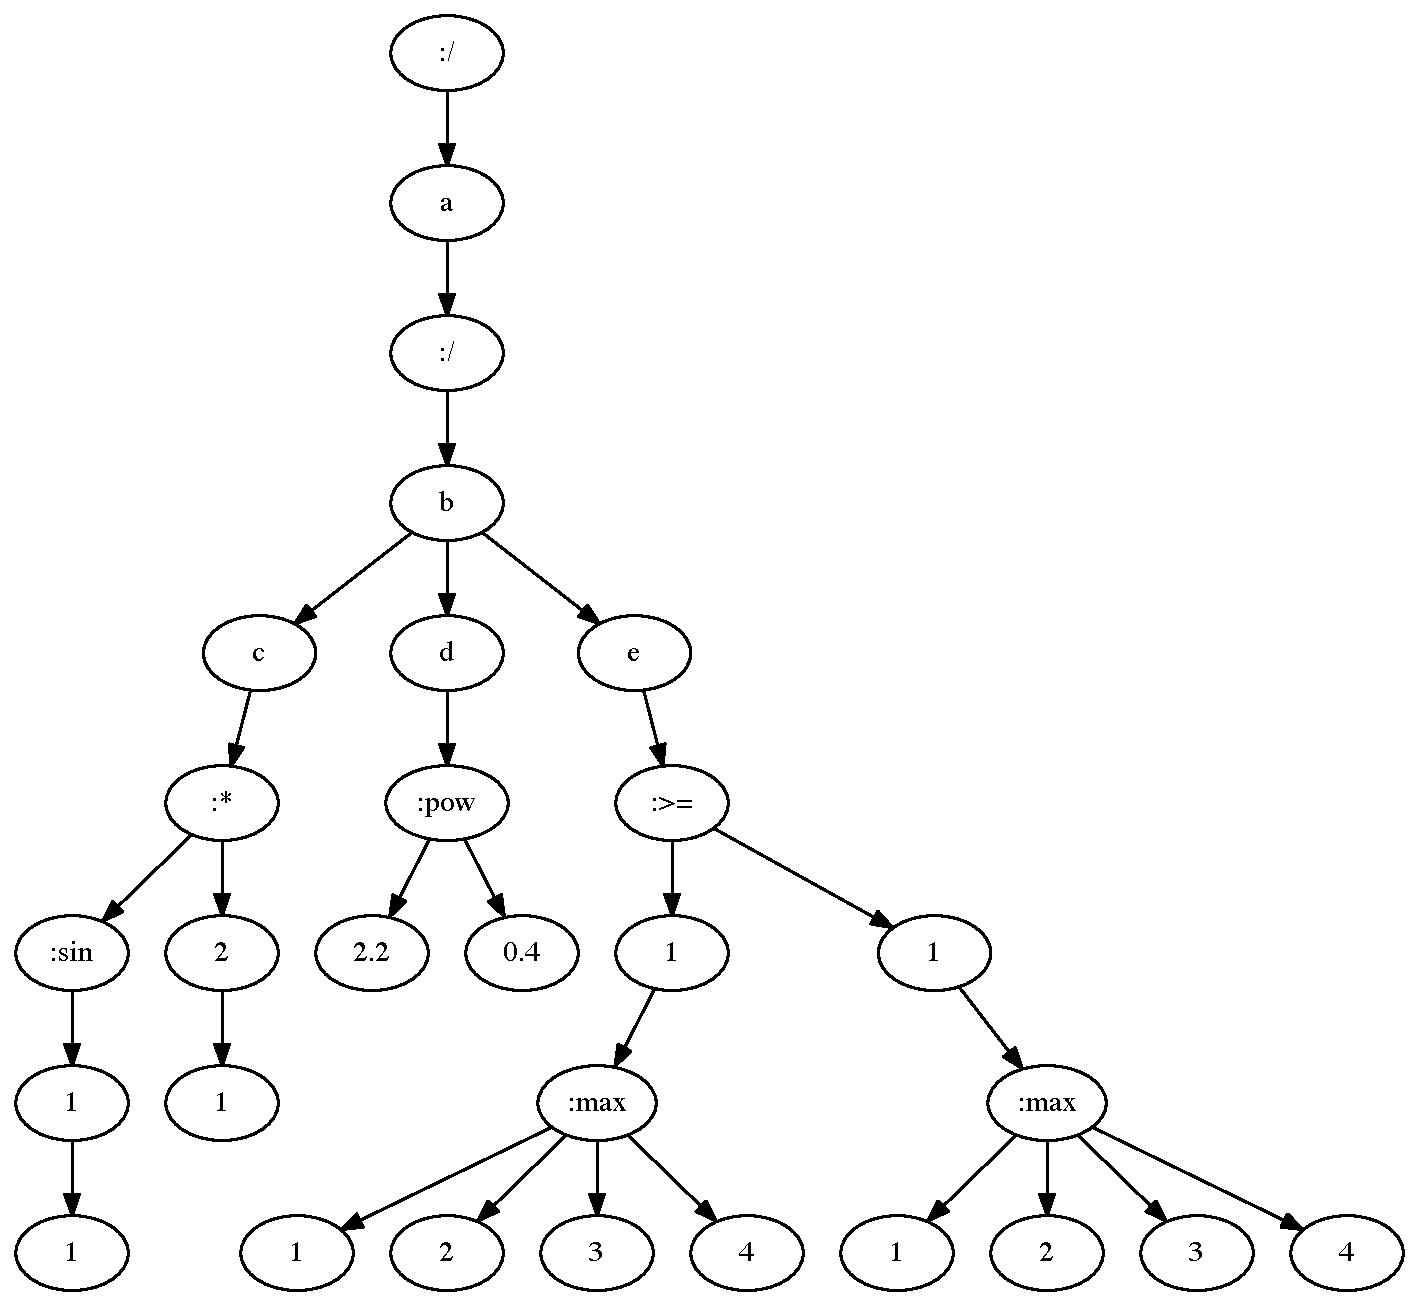
\includegraphics[width=1\columnwidth]{tree/sample3}
\caption{Arbre construit par le script ci-dessus.}
\label{parsesample2}
\end{center}
\end{figure}

\begin{figure}[htbp]
\begin{center}
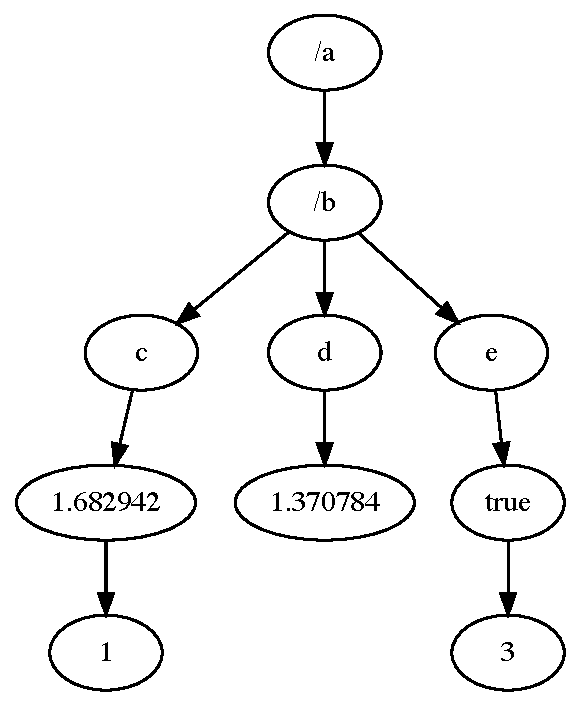
\includegraphics[width=0.62\columnwidth]{eval/sample3}
\caption{Arbre généré après évaluation des opérations mathématiques de l'arbre en figure \ref{parsesample2}.}
\label{treesample2}
\end{center}
\end{figure}


%---------------------------
%\subsubsection{Sélecteurs}
%
%Un sélecteur est un arbre qui prend la forme suivante :
%\code{? condition, if\_true, if\_false}
%Il sélectionne une des deux branches en fonction de la valeur booléenne de la \emph{condition}.
%
%\exemple
%
%Une fois évalué, le script illustré en figure~\ref{dotselect} sera réduit à l'arbre $t : 1\ [\nulltree]$.
%
%\begin{figure}[htbp]
%\code{? true, 1, 0;}
%\begin{center}
%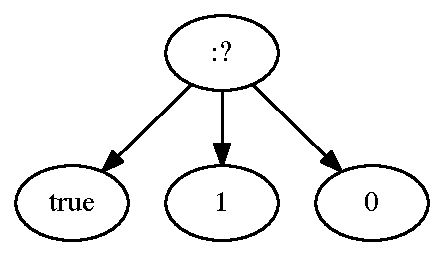
\includegraphics[width=0.5\columnwidth]{tree/select}
%\caption{Arbre construit par le sélecteur ci-dessus. En regard de la valeur du premier enfant, son évaluation va sélectionner la branche 1.}
%\label{dotselect}
%\end{center}
%\end{figure}
%


%---------------------------
\subsection{Variables}

Le type de valeur \emph{variable} désigne un arbre dont la valeur fait référence à un autre arbre.
L'évaluation d'un arbre variable consiste à développer l'arbre référencé à la position variable.
Définissons une variable $var$ et un arbre variable $t'$ comme suit :
\[
\left\{
\begin{array}{l}
	var = v \times \llist{t} \\
	t' : \$var \times \llist{t'}\\
\end{array}
\right.
\]
alors 
\[
	t'_{\{var\}}  \to v \times \llist{t}\ \seq\ \forest \times \llist{t'}
\]
t'$_{\{var\}}$ représente l'arbre $t'$ dans un environnement contenant la définition de la variable $var$.


\exemple
\code{x = x 0;\\
y = y 0;\\
/A/B \$x, \$y; \ \ $\Rightarrow$  /A/B (x 0), (y 1);}


%---------------------------
\subsubsection{Environnement local à une variable}

Chaque arbre est évalué dans un environnement constitué de la liste de toutes les variables de son parent. Cependant, une variable peut-être évaluée dans un environnement qui lui est local. Les variables locales sont définies entre accolades :
\[
\left\{
\begin{array}{l}
	var = t \\
	\$var\{a=t1, b=t2,\etc\} \ \to  t_{\{a, b,\etc\}} \\
\end{array}
\right.
\]


%---------------------------
\subsection{Valeurs expansées}

Une \emph{valeur expansée} est une forme compacte de description d'une forêt. On peut les voir également comme une manière de décrire des boucles. Leur forme syntactique est la suivante :
\begin{description}
\item $id[n…m]$ 	où $n$ et $m$ sont des entiers
\item $id[ab…xy]$ où $a,b,x,y$ sont des lettres.
\end{description}
Nous noterons \nexpand\ l'opération d'expansion :
\[
\left\{
\begin{array}{l}
	\nexpand(id[n\etc m])   \ \ \to \forest \ [id_n,id_{n+1},\etc ,id_m] \\
	\nexpand(id[ab\etc xy]) \to \forest \ [id_{ab},id_{ac},\etc ,id_{ay}, \\
	\ulb \etc ,\\
	\ulb id_{xb},id_{xc},\etc ,id_{xy}]
\end{array}
\right.
\]
où chaque $id_n$ est un arbre $v \times \emptyf$ dont la valeur $v$ est la concaténation de la valeur de base $id$ et de l'index courant $n$.

%---------------------------
\subsubsection{Formes particulières}

Une \emph{valeur expansée} peut également prendre les formes particulières suivantes : 
\begin{description}
\item $id[i:n…m]$ 	où $i$ est un identificateur
\item $id[i:j:ab…xy]$ où $i,j$ sont des identificateurs.
\end{description}
Ces identificateurs désignent des variables qui sont instanciées dans l'environnement par l'opération d'expansion, avec la valeur d'indice courante, i.e.:
\[
%	\nexpand(id[i:n\etc m]) \to \forest \ [id_{n\{i=0\}},id_{n+1\{i=1\}},\etc ,id_{m\{i=m-n\}}] \\
	\nexpand(id[i:n\etc m]) \to \forest \ [id_{n\{i=0\}},\etc ,id_{m\{i=m-n\}}] \\
\]


%---------------------------
\section{Conversion en OSC}\label{ssec:slash}

Un message OSC est constitué d'une adresse OSC (similaire à un chemin Unix) suivie d'une liste de données (qui peut éventuellement être vide)
La valeur spéciale \emph{slash} d'un arbre est utilisée pour distinguer l'adresse OSC et les données. Pour ce faire, nous allons \emph{typer} les valeurs et nous définissons \taddress\ comme le type d'une valeur faisant partie d'une adresse OSC. Nous noterons $\type(v)$ pour faire référence au type de la valeur $v$.

Nous noterons $t^a$ pour désigner un arbre $t$ dont la valeur est de type \taddress\ .
Ensuite, nous définissons une opération \toAddress\ qui transforme un arbre en arbre \emph{typé} :
\[
    \toAddress (v \times \llist{t}) \to 
\left\{
\begin{array}{l}
	\forest \times \llist{t^a} , v = /\\
	v \ \times \llist{t} , v \neq / \\
\end{array}
\right.
\]

La conversion d'un arbre $t$ en messages OSC transforme l'arbre typé $\toAddress (t)$ en une forêt d'adresses OSC suivies de données :\\

%\[
%    \toOSCAddress (v \times \llist{t}) \to
%\]
\vspace*{2mm}
\hspace*{5mm} $\toOSCAddress (v \times \llist{t}) \to$
\[
\left\{
\begin{array}{l}
	\forest \times [ v \times \toOSCAddress(t_1),\etc , v \times \toOSCAddress(t_k)] , \type(v) = \taddress\\
	v \ \times [ \toOSCAddress(t_1),\etc , \toOSCAddress(t_k)] , \hspace{12mm} \type(v) \neq \taddress \\
\end{array}
\right.
\]

La figure \ref{pathssample4} donne une exemple de transformation d'un arbre en chemins OSC.
\begin{figure}[htbp]
\begin{center}
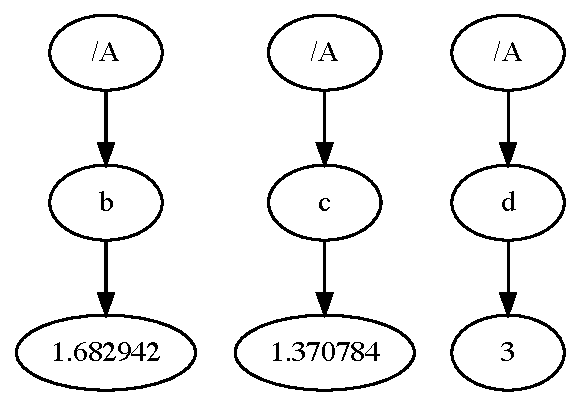
\includegraphics[width=0.6\columnwidth]{paths/sample3}
\caption{Transformation de l'arbre de la figure \ref{treesample2} en chemins OSC.}
\label{pathssample4}
\end{center}
\end{figure}


%-------------------------------------------------
\section{Exemple de script}

Le script ci-dessous présente un exemple de cette nouvelle version du langage \IS . Les variables sont indiquées en bleu, les variables locales sont déclarées en rouge.

\lstdefinelanguage{inscore} 
{
classoffset=0,
morekeywords={}, keywordstyle=\color{blue},
classoffset=1,
morekeywords={addr, count, radius, size, pos, color }, keywordstyle=\color{red},
classoffset=2,
keywordsprefix=$,
sensitive=true,
morecomment=[l]{\#},
morestring=[b]", 
}

\lstset{backgroundcolor=\color{lightgrey}, extendedchars=true, inputencoding=utf8}

\begin{lstlisting}[language=inscore, extendedchars=true, basicstyle=\small\ttfamily]
# variables declaration 
pi    = 3.141592653589793;

# the 'step' variable makes use of 'count'
# a variable that is instantiated locally
step  = / ( * 2, $pi), $count;

# the variable 'i' is defined by the 
# expansion of the address 'n_[i:1...9]'
x = math.sin ( * $step, $i );
y = math.cos ( * $step, $i );

# the following variables select part of
# guido music notation code to 
# build a short score
dyn = (? (% $i, 3), '\i<"p">', '\i<"ff">');
note = (+ $dyn, " ", (?  (% $i, 2), 
	"e2", 
	"g1/8"));

# this is a classical OSC message
# that simply clears the scene
/ITL/scene/* del;

# this is the main variable. It will be
# expanded to create a series of small 
# scores. The variables are computed 
# using locally defined variables.  
notes = (/ITL/scene/$addr  
	(set gmn (+ "[", $note, "]")),
	(scale 0.7),
	(x * $x, $radius),
	(y * $y, $radius)); 

# finally the 'notes' variable is used 
# addr, count and radius are local.
# which could be viewed as a function call
$notes{ addr=n_[i:1...9], 
        count=9, 
        radius=0.7};
\end{lstlisting}



L'évaluation de ce script produit des messages OSC pleinement compatibles avec la version précédente du langage et qui sont schématiquement présentés ci-dessous. 
\code[1]{//ITL/scene/n\_1 set gmn '[ \i<"ff"> g1/8]';\\
/ITL/scene/n\_1 scale 0.7;\\
/ITL/scene/n\_1 x 0.0;\\
/ITL/scene/n\_1 y 0.7;\\
/ITL/scene/n\_2 set gmn '[ \i<"p"> c2]';\\
/ITL/scene/n\_2 scale 0.7;\\
/ITL/scene/n\_2 x 0.411449;\\
/ITL/scene/n\_2 y 0.566312;\\
...\\
...\\
/ITL/scene/n\_9 set gmn '[ \i<"ff"> c2]';\\
/ITL/scene/n\_9 scale 0.7;\\
/ITL/scene/n\_9 x -0.411452;\\
/ITL/scene/n\_9 y 0.56631;
}


Dans la pratique, cet exemple exprime la scène illustrée en figure \ref{samplescene} en quelques lignes seulement.

\begin{figure}[htbp]
\begin{center}
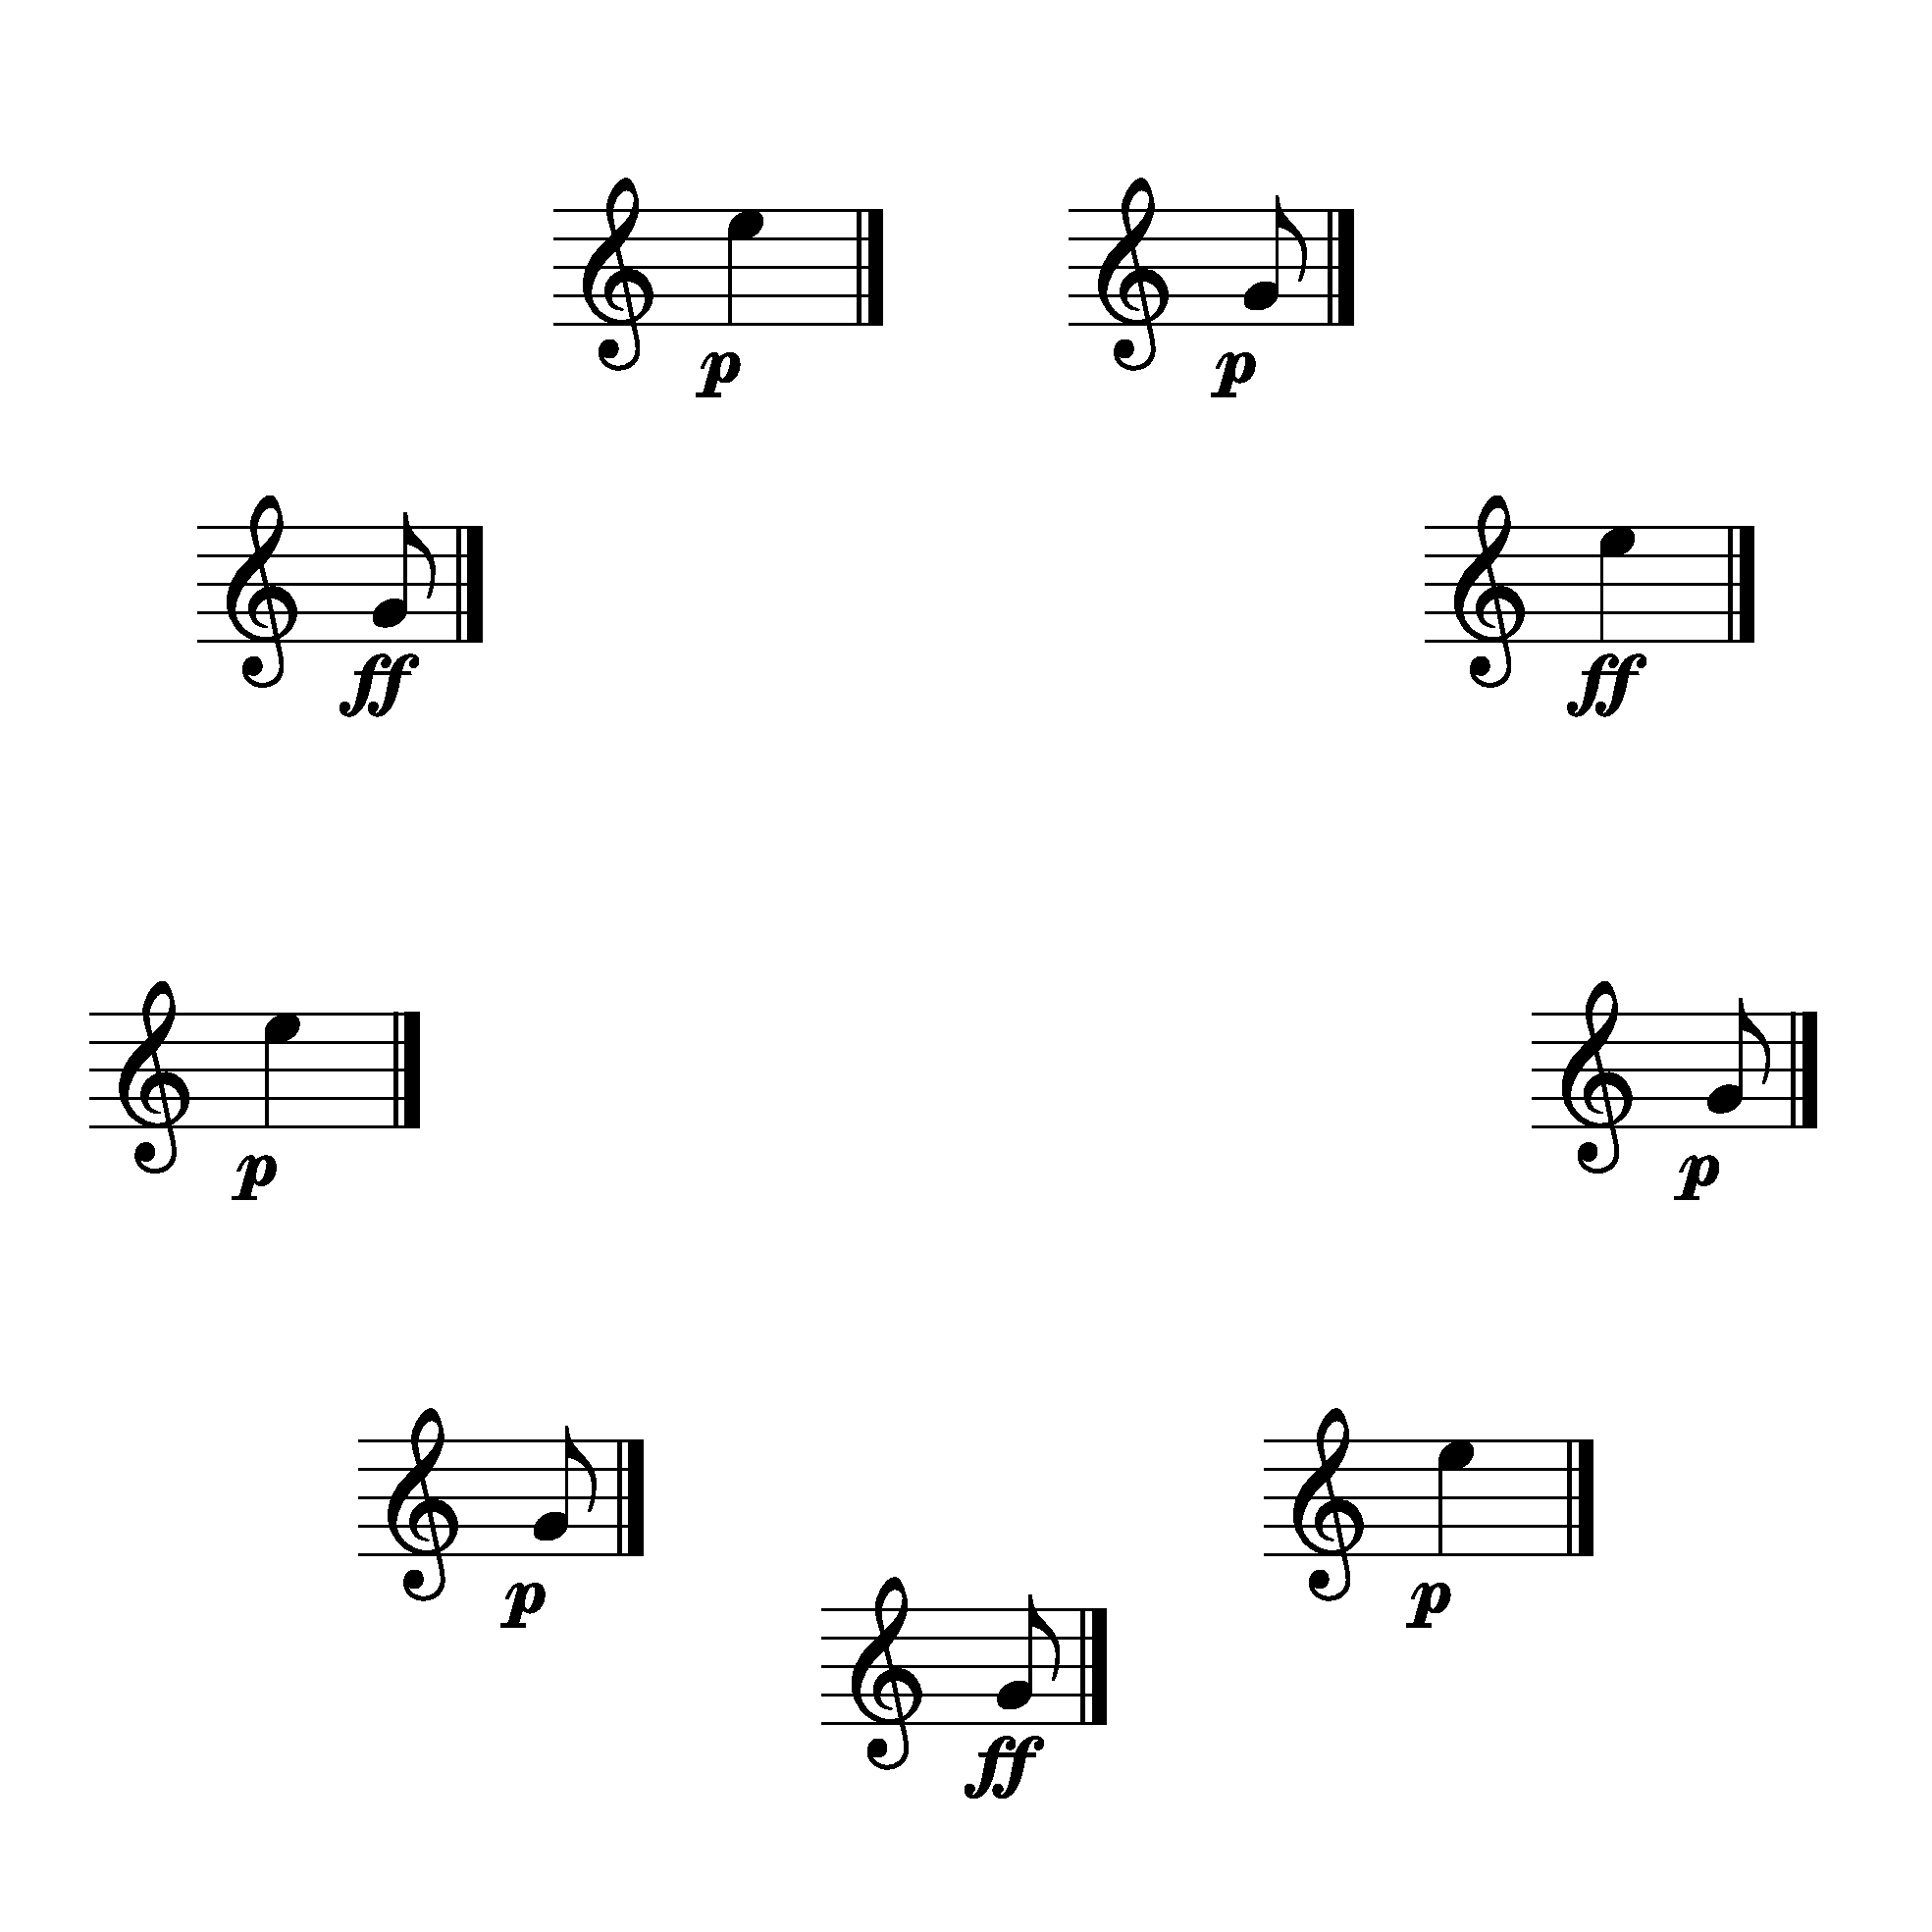
\includegraphics[width=0.98\columnwidth]{scene}
\caption{Partition \IS\ correspondant au script ci-dessus.}
\label{samplescene}
\end{center}
\end{figure}


%==============================================================
\section{Conclusion}

A partir de deux opérations élémentaires sur des arbres - la mise en séquence et en parallèle -, nous avons pu introduire de manière homogène, les notions de variables et d'opérations mathématiques et logiques portant sur des arbres. Le langage résultant est d'une  expressivité sans commune mesure avec la version précédente du langage de script d'\IS . Il permet notamment la mise en parallèle des arguments d'un message, d'utiliser des variables pour décrire des adresses, d'exprimer des séries d'adresses de manière concise, et d'utiliser des variables locales permettant la réutilisation de scripts ou de parties de scripts dans des contextes différents.

\balance
\bibliographystyle{plain}
\bibliography{../interlude}


\end{document}
